%linux boot flow chart
\documentclass{article}
\usepackage{tikz}
\usetikzlibrary{chains}
\begin{document}
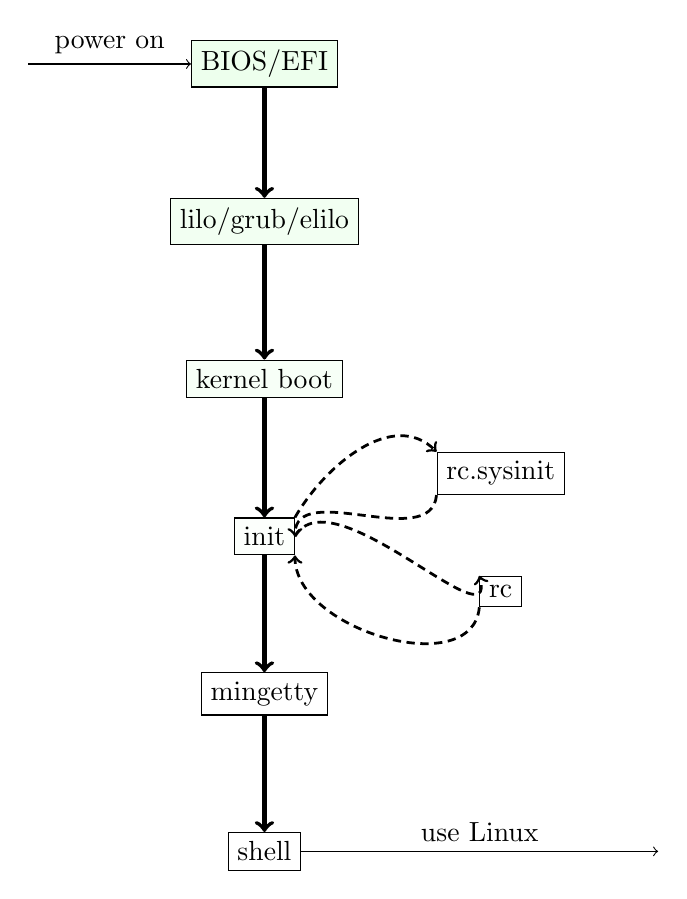
\begin{tikzpicture}[	node distance=10mm,%
					start chain=1 going below,%
					every node/.style=draw,%
					every join/.style=->]
%\tikzstyle{every node}=
%	[%
%		fill=green!50!black!20,%
%		draw=blue!50!black,%
%		minimum size=2cm,%
%		minimum height=8mm,%
%		draw,%
%		thick
%	]
%\node (bios) {BIOS/EFI};
%\node (loader) [below of = bios] {lilo/grub/elilo};
%\node (kernel) [ below of = loader] {kernel boot};
%\node (init) [below of = kernel] {init};
%\node (sysinit) [ right of = init ] {rc.sysinit};
%\node (rc) [ right of = init ] {rc};
%\node (mingetty) [below of =init]{mingetty};
%\node (shell) [ below of = mingetty]{shell};

\foreach \a\b\c\d in { bios/0/7/{BIOS/EFI},grub/0/5/{lilo/grub/elilo},kernel/0/3/{kernel boot} ,init/0/1/init,mingetty/0/-1/mingetty,shell/0/-3/shell}
	\node [fill=green!\c] (\a) at (\b,\c) {\d};
	%\node [draw,on chain=1,join] (\a) {\d};



\node (sysinit) at (3,1.8) {rc.sysinit};
\node (rc) at (3,0.3) {rc};

\foreach \from/\to in {bios/grub,grub/kernel,kernel/init,init/mingetty,mingetty/shell}
	\draw [ ->,line width=1.5pt ] (\from) -- (\to);

\tikzstyle{every node} =[ ] 	

\draw [->] (-3,7) -- (bios) node[pos=.5,sloped,above] {power on};
\draw [->] (shell) -- (5,-3) node[pos=.5,sloped,above] {use Linux};	
	
\path  [densely dashed,->,line width=1pt] (init.north east) edge [out=60,in=135] (sysinit.north west);
\path [densely dashed,->,line width=1pt] (sysinit.south west) edge [out=265,in=90] (init.east);

\path  [densely dashed,->,line width=1pt] (init.east) edge [out=60,in=285] (rc.north west);
\path [densely dashed,->,line width=1pt] (rc.south west) edge [out=265,in=270] (init.south east);

\end{tikzpicture}
\end{document}